\chapter{Empirical Evaluation}
\label{chapter_evaluation}

% **************************** Define Graphics Path **************************
\ifpdf
    \graphicspath{{Chapter5/Figs/Raster/}{Chapter5/Figs/PDF/}{Chapter5/Figs/}}
\else
    \graphicspath{{Chapter5/Figs/Vector/}{Chapter5/Figs/}}
\fi

This chapter explains the empirical evaluation of the methods suggested in chapter \ref{chapter_solutions}. Section \ref{sec_applicationDomain} presents the application domain and the associated dataset. Section \ref{sec_transformation} then follows up with a description of small adjustments to the suggested algorithm as well as transformations applied to the dataset. Subsequently section \ref{sec_evaluationMetrics} explains the choice of evaluation metrics. Finally section \ref{sec_evaluationResults} presents the evaluation results and explains the observations made from the plots.

\section{Application Domain and Dataset}
\label{sec_applicationDomain}

\subsection{Dataset}
As mentioned in the introduction the application domain for the streaming prediction algorithms conceived in this thesis is financial data. Basic approaches and challenges in the forecasting of financial time series have already been covered in the related work chapter (see section \ref{sec_stock_market_prediction}). The dataset was assembled using data provided by the Yahoo Finance website \cite{yahooFinance} The dataset has the following properties:
\begin{itemize}
	\item It contains data about all companies traded at the National Association of Securities Dealers Automated Quotations (NASDAQ), which is the second largest stock exchange of the USA.
	\item The data-set contains tick-data that was sampled at a 15-second interval (meaning Yahoo Finance was polled for the current value every 15 seconds).
	\item Each entry in the dataset is a triple consisting of a timestamp, the company and the current stock-value.
	\item For the purpose of this thesis these companies are filtered by whether they have an entry in the dbpedia \cite{auer2007dbpedia}, which is a commonly used source for semantic knowledge. This reduces the number of companies to 40, however the base dataset still contains all other companies.
	\item The data was sampled from the 9th of May 2016 to the 23. November of September 2016. However, some days in between are missing due to the data being corrupted. In total the dataset contains 48 trading days.
\end{itemize}

\subsection{Data Quality}
\label{subsec_dataQuality}
The yahoo Finance Website is a free to use data source and while it does display the current stock prices, there are no quality guarantees given. Thus there might be errors or inaccuracies in the derived dataset. Thus the evaluation must proceed cautiously, since the quality of the underlying data is unknown. In fact, when examining the values of individual companies in the derived dataset there are sometimes significant jumps from one value to another. The main problem here is that it is impossible to tell whether those jumps are due to errors, or delayed updates on the server side or whether they are caused by large buy or sell actions, for example by high-frequency traders. For this reason the evaluation will consider them in a special manner, once including them and once filtering them out (dismissing them as invalid data) in order to evaluate model performances for both cases (TODO: do we actually still do that? Remove this when the rest of this chapter is finished). 

\subsection{Restrictive Use of Data}
The yahoo finance website offers data for private use only, which unfortunately means that the author of this thesis is not able to publish the dataset obtained by querying the yahoo finance website, as that would be a redistribution of the original data, which is explictly prohibited by the Yahoo Terms of Use \cite{yahooTermsDeveloper}.

\section{Dataset Transformation and Algorithm Adjustments}
\label{sec_transformation}

TODO: 


\subsection{Dataset Transformation}

Since the algorithms introduced in chapter \ref{chapter_solutions} work on event data streams, meaning streams of categorical values (episodes are only defined for categorical event types). Since however the dataset described in section \ref{sec_applicationDomain} in its base form has numerical values, these numerical streams need to be transformed to categorical streams, in which the prediction of a specific event type is of interest. There are many different ways of transforming the numerical data streams, neither of which are necessarily right or wrong. The most simple transformation is a simple comparison of the current value of a stock to the previous value. This produces three different event types per company: \textit{DOWN}, \textit{EQUAL} and \textit{UP}. This will result in a stream with a lot of events, which makes the episode mining task hard, since there is a lot of data to consider. The amount of data can be reduced by discarding events of type \textit{EQUAL}, which are generally less interesting than up or down movements. \\
Another possible way of transforming the data is by doing aggregation until a change of a certain amount can be found (for example at least 1\% of the original value). Aggregation in this form will produce much less annotated events. A disadvantage of this approach however is that the the usefulness of predictions might suffer. This is due to the fact that if events are aggregated over time the UP-event for a company at timestamp $t$ does not mean that its stock suddenly increases at timestamp $t$, but instead means that a gradual increase by 1\% finishes at timestamp $t$. Thus if the model predicts such an Up-event shortly before $t$ and chooses to invest, the net-gain will not be 1\% but probably much less. For these reasons the numerical streams were transformed without aggregation and without considering events of type \textit{EQUAL}.

\subsection{Adjustments to PERMS}
Since we are now in the concrete use-case of predicting stock movements, we need to slightly adjust the PERMS algorithm presented in chapter \ref{chapter_solutions}. Recall that PERMS builds a model to predict one specific event. Say we have a company $C$ and we want to use the output of a predictive model to automatically buy or sell stocks of $C$. There are two events that we need to predict for that, which are $C_UP$ and $C_DOWN$. If we assume that buying or selling stocks does not cost a fee, false positives of the models with the stock value of $C$ remaining equal do not hurt the investment. \\
Instead of building two models we slightly adjust the window mining process as shown in figure TODO.

 TODO: how the hell do I describe what I did in PERMS??

\subsection{Adjustments to FBSWC}
The FBSWC algorithm does not need to be changed as much, the only thing that changes, is that for a company $C$ the classification task is no longer binary. Instead there are now three classes: $\{UP,EQUAL,DOWN\}$. Like in the adjustment to PERMS positive, neutral and negative windows can be mined from the stream and used as training examples for the feature based classifier. \\
As a feature based classifier, the random forest was chosen, since it offers good classification time and can be adjusted to work with incremental updates, should one consider to evolve the model as the stream progresses.\\
Also a feature selection approach must be chosen. A simple but effective approach is continous feature selection using Filter-Schemes \cite{molina2002feature}, in which features are assigned weights based on their usefulness (according to some measure). Afterwards the features are ranked according to their weights and the best are chosen. In the experiments that were done in Chapter , the continous feature selection using the Filter-Scheme with information gain (TODO: define information gain) as a measure was used. As a feature based classifier a random forest was used.

\section{Evaluation Metrics}
\label{sec_evaluationMetrics}

In order to evaluate the quality of predictive models and thus reach conclusions about the original algorithms, appropriate evaluation metrics need to be chosen. The domains of both machine learning as well as stock market prediction offer diverse metrics that can be used to determine the quality of models. The most important quality metrics and their usage in this context will be discussed in the following subsections.

\subsection{Test Examples}
In order to make use of evaluation metrics, we must first clarify how we test the model, and what exactly qualifies as a test-example. For this, recall that the predictive models take the current state of the stream (defined as the current window) and will then output a prediction of whether the target event will follow after this window. Since the Window-size is fixed in duration, we can obtain a sliding window over the stream, starting at the position, where we finished scanning the stream for training data (see subsection \ref{subsec_perms}, algorithm \ref{alg_traningExampleMining}). From then on we can slide the window forward as new events are coming in and use each individual window as a test example, that we test the model on. This is visualized in figure \ref{fig_testData}.

\begin{figure}[h]
	\centering
  	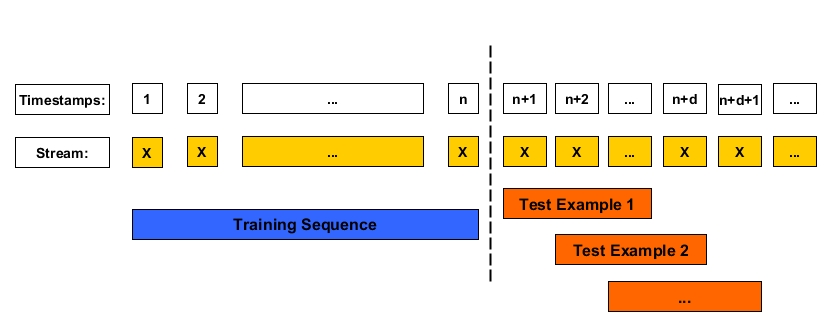
\includegraphics[width=0.75\textwidth]{testData}
	\caption{Test Example Collection for evaluating the models}
	\label{fig_testData}
\end{figure}

\subsection{Rate of Return and Investment Strategies}
\label{subsec_investmentStrageties}
Before we can talk about the rate of return we must first understand simple investments, that can be made at a stock market. There two basic events that are relevant: The stock of a company can rise or fall. For each of these there is an appropriate investment. \\
Let us say an investor predicts a rise in stock value. In this case the investor will buy one of the stocks and then sell it after the price has risen, which leaves the investor with the price difference as a net-gain. In financial jargon this is also called a long investment, or simply long. \\
If however the stock price is expected to fall, it is still possible to make profit by doing the following: First the investor borrows stocks from someone and then immediately sells them for the current price. Then after the price has fallen, the investor buys the stocks for the now lower price and gives them back to the lender. Once again the investor makes profit based on the price difference, assuming the lender does not require the investor to pay a fee. This sort of investment is called a short investment, or simply short. \\
There are a few things to note here:
\begin{itemize}
	\item It is easy to see that if the investor's prediction is incorrect he or she will lose money. The loss is also equal to the difference between current and future stock value.
	\item Shorts usually require an additional fee, that needs to be payed to the lender for borrowing the stocks. However in this evaluation we will assume that such a fee does not exist.
\end{itemize}

Having explained the basic types of investments, it is easy to create an investment strategy based on the model's predictions. This investment strategy is depicted in algorithm \ref{alg_investmentStrategy}. 

\begin{algorithm}[H]
  \caption{Investment Strategy
    \label{alg_investmentStrategy}}
  \begin{algorithmic}[1]
    \Statex
    \Require Let $M$ be the predictive Model, $W$ the current window of the Stream and $t$ the time delay.
    \Function{WindowMining}{}
      	\If{$M(W) = UP$}
      		\State make a long investment, re-sell Stock $t$ seconds later
		\ElsIf{$M(W) = DOWN$}
			\State make a short investment, re-buy Stock $t$ seconds later
       	\EndIf
    \EndFunction
  \end{algorithmic}
\end{algorithm}

It is a very basic strategy that entirely relies on the model output. The only remaining parameter to determine is $t$, the time at which we want to re-sell (in case of longs), or re-buy (in case of shorts) the stocks. Recall that in the training process of the models, we select our examples, by cutting off the window just before the target event, meaning we train the model to recognize situations, in which the next incoming event is the target event. Thus in the general case $t$ should be set to the expected time difference between two timestamps in the stream. Of course, not all streams have a constant update rate in which case things get more complicated. For this specific dataset however, we know that the stream is sampled at a 15 second interval, which is why we set $t = 15s$. \\
After having defined how investments are made, we can finally define the rate of return for an investment. Given the $S$ as the amount of money that was invested, and $E$ as the amount of money left after the investment the rate of return is defined as $r = \frac{E-S}{S}$. As models are being evaluated as described in the previous subsection, many investments will be made, which is why we can define the total rate of return for a model as the sum of all the individual returns that are obtained during the model evaluation.\\
There are a few assumptions, that we need to make in order for this to work. these are:

\begin{itemize}
	\item Short or long investments can be made at any time and they can be made instantaneously.
	\item Making these investments has no influence on the stock price.
	\item Making these investments has no additional cost.
\end{itemize}

Depending on the scenario these assumptions can be more or less realistic and it is important to keep that in mind when looking at the model's rate of return. They will probably not translate one to one to the real world. Apart from that, the rate of return is representing the ground truth about a model, given that the underlying data is valid. The higher the rate of return, the better is the model.

\subsection{Accuracy, Precision and Recall}
The way that the prediction of the stock movement is tackled in this thesis is essentially a three-class classification problem. The value of a stock can either rise, fall or remain equal. It is also clear, that for all test examples, we know the actual class, which means that we can record all test results in a confusion matrix, as shown in figure \ref{fig_confusionMatrix}.
\\
\begin{figure}[h]
\centering
\begin{tikzpicture}[
box/.style={draw,rectangle,minimum size=2cm,text width=1.5cm,align=left}]
\matrix (conmat) [row sep=.1cm,column sep=.1cm] {

\node (tpos) [box,
    label=left:\( \mathbf{UP} \),
    label=above:\( \mathbf{UP} \)
    ] {$U_{U}$};
&
\node (fneg) [box,
    label=above:\textbf{EQUAL}] {$U_{E}$};
&
\node (fneg2) [box,
    label=above:\textbf{DOWN}] {$U_{D}$};
\\


\node (fneg3) [box,
    label=left:\textbf{DOWN}] {$E_{U}$};
&
\node (tpos2) [box] {$E_{E}$};
&
\node (fneg4) [box] {$E_{D}$};
\\

\node (fneg5) [box,
    label=left:\textbf{DOWN}] {$D_{U}$};
&
\node (fneg6) [box] {$D_{E}$};
&
\node (tpos3) [box] {$D_{D}$};

\\
};
\node [left=.05cm of conmat,text width=1.5cm,align=right] {\textbf{actual \\ value}};
\node [above=.05cm of conmat] {\textbf{prediction outcome}};
\end{tikzpicture}
\label{fig_confusionMatrix}
\caption{Confusion Matrix example}
\end{figure}

The classical evaluation metrics accuracy, precision and recall can now easily be applied to this scenario. We briefly repeat their definitions here:
TODO: define accuracy precision, recall, talk about leaving out equal

\subsection{Corrected Return}
As mentioned in subsection \ref{subsec_dataQuality} the correctness of the underlying data can not be guaranteed. The fact that there are some significant jumps in stock values may hint at errors in the data in some cases, however it is also plausible that this is in fact normal, volatile behavior of the stock market. In order to account for possible errors, we can define an additional metric, called the corrected return. The corrected return works just like the normal return, except that we exclude test examples in which there was a subsequent increase or decrease by more than $5\%$ of the original value. It is important to keep in mind that this does most likely not represent the true performance, however it does have the benefit of filtering out large outliers. Thus the corrected return can serve as a heuristic that describes how the model would have performed, if the stock value was less volatile.

\section{Evaluation Result}
\label{sec_evaluationResults}

\subsection{Explorative Analysis}

As a first exploratory analysis the following configuration was selected for the algorithms:

\begin{itemize}
	\item $d = 90s$
	\item $m = 100$ 
	\item $s_P = 0.8$
	\item $s_S = 0.8$
	\item $n = 20$ (only relevant for PERMS)
\end{itemize}

A Model was trained for each approach and for each company, resulting in 80 different models, using this configuration. Figures  \ref{fig_firstRunReturnByCompany} and \ref{fig_firstRunCorrectedReturnByCompany} show the rate of return and corrected rate of return for each model.

\begin{figure}[h]
	\centering
  	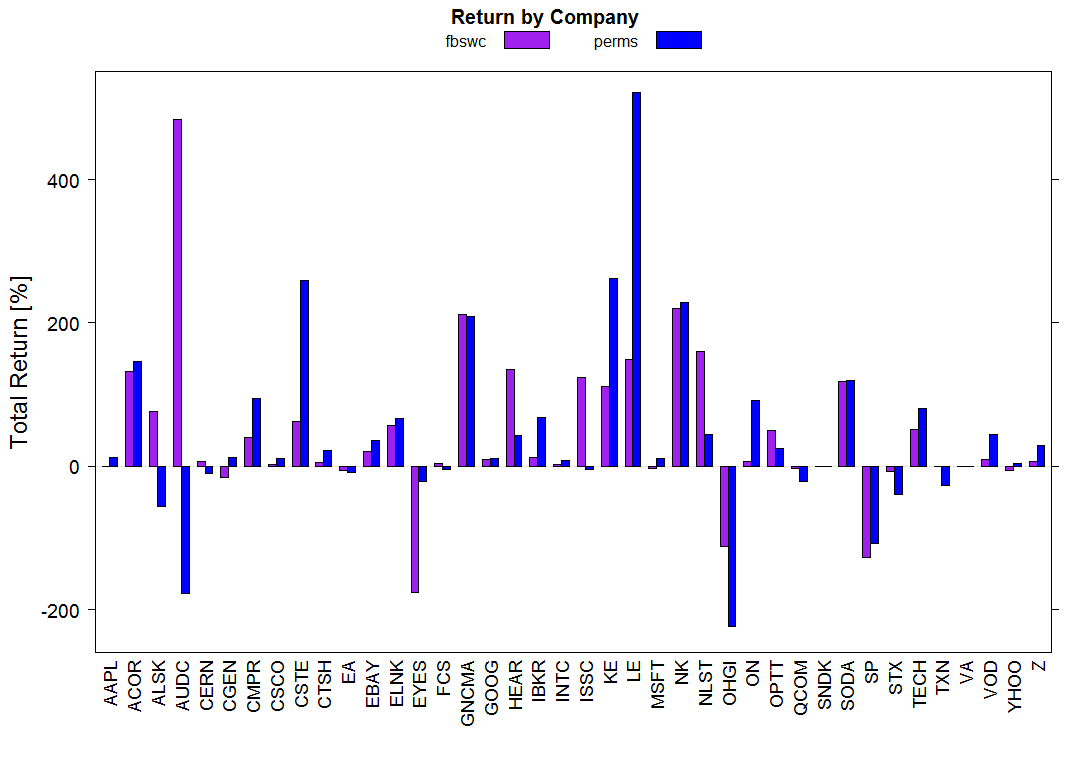
\includegraphics[width=0.75\textwidth]{firstRunReturnByCompany}
	\caption{Histogram: Rate of Return}
	\label{fig_firstRunReturnByCompany}
\end{figure}

\begin{figure}[h]
	\centering
  	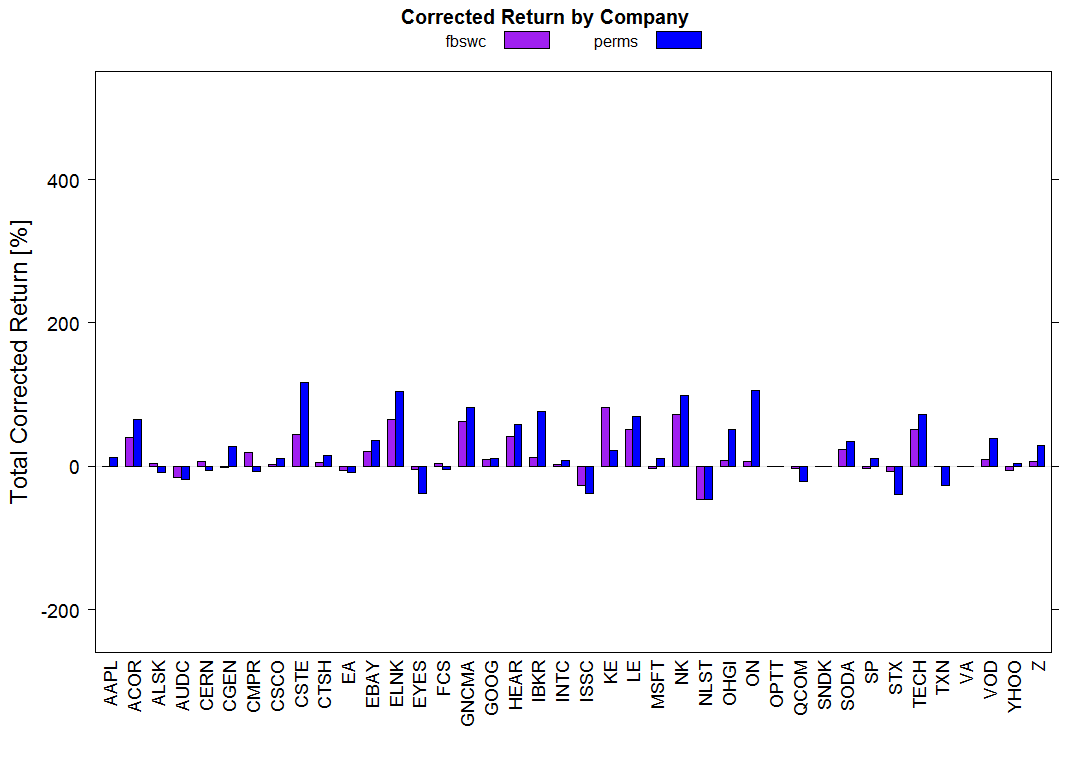
\includegraphics[width=0.75\textwidth]{firstRunCorrectedReturnByCompany}
	\caption{Histogram: Corrected Rate of Return}
	\label{fig_firstRunCorrectedReturnByCompany}
\end{figure}

Both histograms show that there is quite a large disparity between the different models for the different companies. Table \ref{table_firstRunReturn} shows the average return values over the models, as well as the standard deviation.

\begin{table}
\label{table_firstRunReturn}	
\caption{Mean and STD of the model's Return}
\begin{tabular}{ c | c | c | c | c}		
  Model Type & mean(Return)  $[\%]$ & std(Return) $[\%]$ & mean(Corrected Return) $[\%]$ & std(Corrected Return) $[\%]$ \\
  \hline
  PERMS & 44.0 & 124.3 & 22.9 & 27.1\\
  FBSWC & 45.4 & 107.3 & 13.4 & 43.3\\
\end{tabular}
\end{table}

 The first thing to note here is that the mean values of 0.44 and 0.45 for return are extremely high. This essentially means that on average, automatic trading algorithms using the models built by the methods suggested in this paper would make a profit of $44\%$ or $45\%$ respectively. Even for the much lower values of corrected return, which filters out outliers, the models still achieve $22\%$ and $13\%$ respectively. These would be amazing results in a real-life scenario. However there are a few things to be noted here. First of all, the standard deviation is higher than the actual mean in all cases, meaning there is a large variance in model performance. A look at the boxplots in figure \ref{fig_returnBoxplot} confirms this.
 
\begin{figure}[h]
\centering
\begin{subfigure}{.5\textwidth}
  \centering
  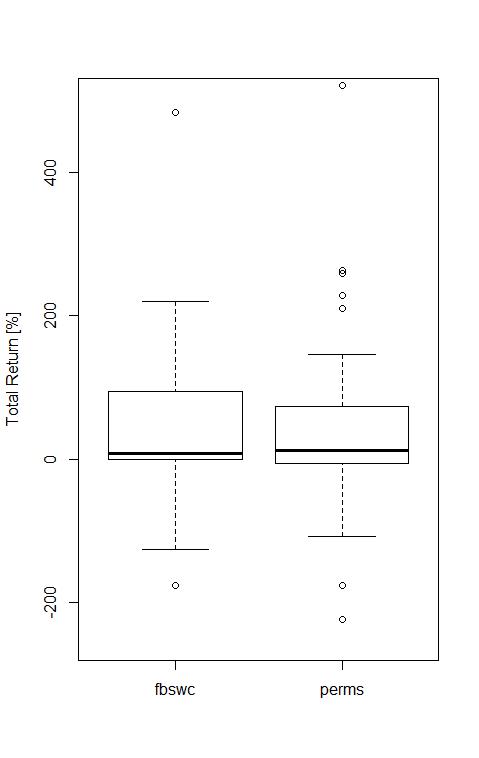
\includegraphics[width=\linewidth]{boxplotReturn}
  \label{fig_returnBoxplot}
  \caption{Return}
\end{subfigure}%
\begin{subfigure}{.5\textwidth}
  \centering
  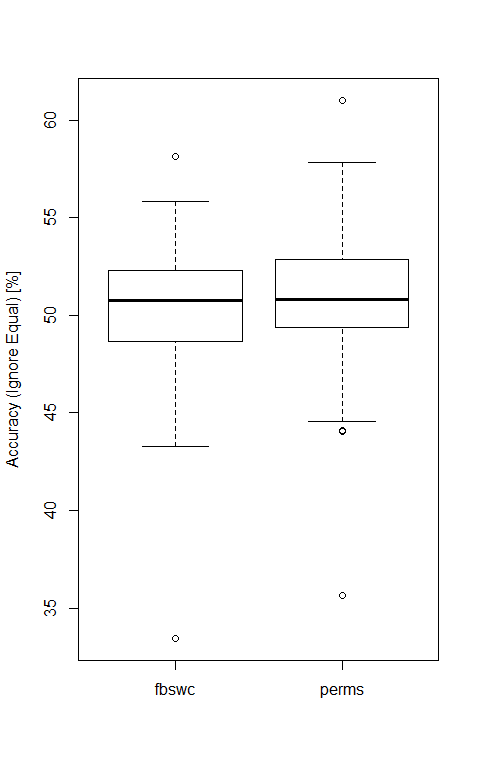
\includegraphics[width=\linewidth]{boxplotAccuracy}
  \label{fig_accuracyBoxplot}
  \caption{Accuracy}
\end{subfigure}
\caption{Boxplots for Return and Accuracy, grouped by Model Type}
\label{fig_returnBoxplots}
\end{figure}

These plots seem to suggest that the algorithms produce models with a high range of quality, either being outstanding like the FBSWC-model for the stock of \textit{AUDC} or extremely weak, like the PERMS-model for the stock of \textit{OHGI}. This seems rather weird, but could be explained by some stocks being easier to predict than others. However, when looking closer at the classical evaluation metrics for classification, it becomes clear, that something is amiss. Figure \ref{fig_accuracyByCompany} plots the accuracy values (ignoring equal events and misclassifications as equal as described in TODO) for the different models. 

\begin{figure}[h]
	\centering
  	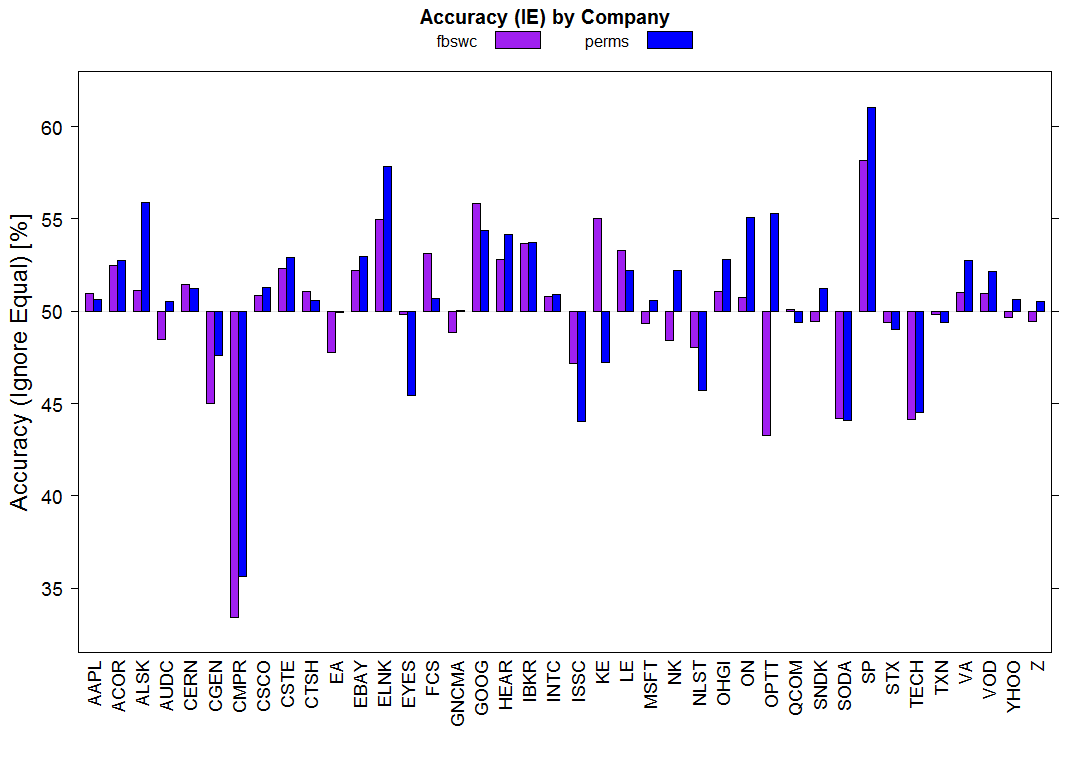
\includegraphics[width=0.75\textwidth]{accuracyByCompany}
	\caption{Histogram: Accuracy (Ignore Equal)}
	\label{fig_accuracyByCompany}
\end{figure}

The origin of the x-axis is set to $50\%$ accuracy, since this is essentially the border we want to overcome. A model with above $50\%$ accuracy is expected to make profits, a model below $50\%$ accuracy is expected to make losses. At first the plot seems to be somewhat consistent with earlier observations, since a majority of models is above $50\%$ accuracy. However, when taking a closer look, it becomes clear that these two metrics contradict each other. Consider the stocks of \textit{CMPR} for example. The accuracy values for both models are extremely poor, however both models apparently net profits, as shown in figure \ref{fig_firstRunReturnByCompany}. One quickly notices similarly weird examples, like the model for the stock \textit{SP}, which performs well accuracy-wise, but nets losses, as shown in the return metric. Additionally the accuracy distibution as shown in table \ref{table_firstRunAccuracy} and boxplot \ref{fig_accuracyBoxplot} has a rather low variance, compared to the return metric.

\begin{table}
\label{table_firstRunAccuracy}	
\caption{Mean and Standard Deviation of the model's Accuracy}
\begin{tabular}{ c | c | c}		
  Model Type & mean(Accuracy) $[\%]$ & std(Accuracy) $[\%]$\\
  \hline
  PERMS & 50,7 & 4,3\\
  FBSWC & 50,0 & 4,1\\
\end{tabular}
\end{table}

 So if the accuracy varies very little, how is it possible that the rate of return is so different for many models? Furthermore, the mean accuracy is actually only slightly above $50\%$ for PERMS and exactly $50\%$ for FBSWC. This can simply not explain an average return of $44\%$ or $45\%$? This discrepancy brings a useful thought to mind: What return would we actually expect the model to have, based on its performance recorded in the confusion matrix? \\

\subsection{Expected Return and Deviation Analysis}
If given the confusion matrix of a model and the time series of the corresponding stock value, we can easily estimate what return we would expect from the automatic investment algorithm explained in subsection \ref{subsec_investmentStrageties}. Lett $TP$ be the number of true positives, (Up correctly classified as UP), $FP$ be the number of false positives (DOWN incorrectly classified as UP), $FN$ be the number of false negatives (UP incorrectly classified as DOWN) and $TN$ be the number of true negatives (DOWN correctly classified as DOWN). Furthermore let $TS = [v_1,...v_n]$ be the time series of stock values. We define $D = [d_1,...,d_{n-1}]$, where $d_i = v_{i+1} - v_i$ as the difference vector of $TS$. Furthermore let $D^+ = [v1,...v_m]$, where $v_i \in D \land v_i > 0$ and let $D^- = [w1,...w_o]$, where $w_i \in D \land w_i < 0$.  Then we can define the average increase as \[INC  = \frac{\sum_{d \in D^+} d}{|D^+|} \] TODO: DIVIDE BY SIZE and the average decrease as \[ DEC = |\frac{\sum_{\substack{d \in D^-}} d}{|D^-|}| \]
With that we can define the expected return as \[ER  = TP \cdot INC + TN \cdot DEC - FP \cdot DEC - FN \cdot INC \]

